\documentclass[11pt, a4paper, twoside, titlepage]{article}
\usepackage[utf8]{inputenc}
\usepackage[a4paper]{geometry}
\usepackage{french}
\usepackage{graphicx}
\usepackage{caption}

\geometry{hscale=0.75,vscale=0.75,centering}
\font\titlefont=cmr12 at 21pt
\graphicspath{ {images/} }

\begin{document}


\title{{\titlefont Projet d'architecture matérielle}\\ARMAgeddon\thanks{J'aime les jeux de mots}}
\author{Pierre KOEBELIN}
\date{\today} 
\maketitle


\begin{abstract}

	L’objectif de ce projet était la réalisation d’un mini-processeur dans Diglog. Pour ce faire, nous devions nous appuyer sur le jeu d'instructions d'un processeur MIPS, que nous avons implémenté dans le logiciel Diglog\ldots\\
\\

\end{abstract}

\tableofcontents

\newpage
\section{ALU}

\begin{center}
	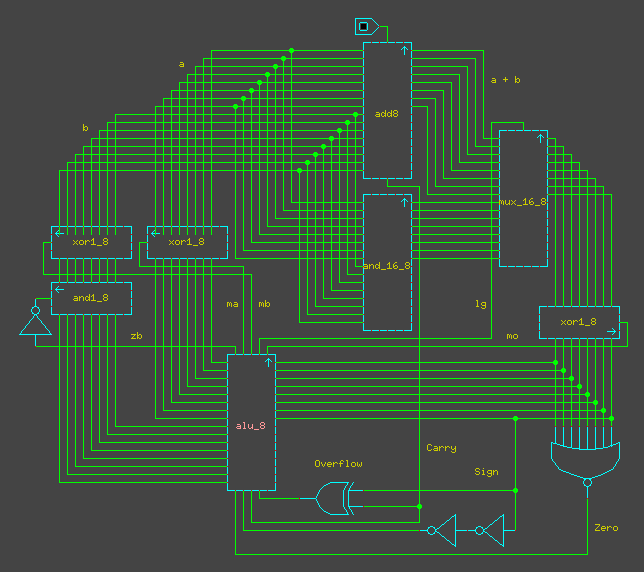
\includegraphics[width=0.8 \textwidth]{alu_8}
	\captionof{figure}{ALU à 5 bits de contrôle et 4 bits de sortie}
\end{center}

\subsection{Bits de contrôle}
Ces bits de contrôle permettent de réaliser différentes opérations sur les entrées \texttt{a} et \texttt{b}.
\subsubsection{zb}
\subsubsection{ma}
\subsubsection{ma}
\subsubsection{lg}
\subsubsection{mo}

\subsection{Bits de sortie}


\newpage
\section{Codes de tests}


\newpage
\section{Modifications apportées au processeur}


\subsection{Implémentation des prédicats}


\newpage
\section{Modifications apportées au compilateur}

\subsection{Gestion des prédicats}

\end{document}